\label{unit2}
% Loading Data into MultiSeq
% bkd 8/2 - I believe this warrants having its own section since there 
%are multiple ways of doing this. i.e., Import Data
% Detail doing a BLAST search

\section{Using and Managing Data}
To begin analyzing proteins in MultiSeq, data from
sequence\footnote{FASTA files.} and
structure\footnote{The ASTRAL database (http://astral.stanford.edu) is a
compendium of protein domain structures derived from the PDB database.
It divides each protein structure into its domain components. For
example, AspRS is divided into three separate PDB files: one containing
the catalytic domain, one with the insertion domain, and one for the
anticodon binding domain. The names of the files contain the PDB
extension, the letter a for ASTRAL, and a number, which corresponds to
which domain it is in the original PDB file.  
%FASTA format is writing a sequence into basic text, such that the sequence can be used to conduct searches via programs like BLAST.
%The Protein Data Bank (PDB) is an archive of experimentally determined three-dimensional structures of biological macromolecules, serving a global community of researchers, educators, and students. The archives contain atomic coordinates, bibliographic citations, primary and secondary structure information, as well as crystallographic structure factors and NMR experimental data.
The PDB is the single worldwide repository for the processing and
distribution of 3-D structure data of large molecules of proteins and
nucleic acids.} files is required.  Import Data (from the File menu
within MultiSeq) allows you to load
structure and sequence files, both locally and via a network connection.

Various structure and trajectory files, such as PDB and PSI, can be
loaded via the \textsf{New Molecule} function of the VMD Main window,
but \textsf{Import Data} allows you to load sequence files as well.
Additionally, Import Data has BLAST searching capabilities, if a local
copy of BLAST is installed.  

\begin{figure}[here]
 \centerline{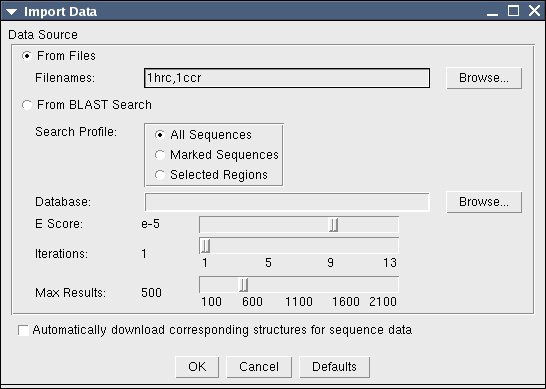
\includegraphics [width=5in]{./pictures/import_data.jpg}}
 \caption{Import Data Window}%more information in caption about views etc.
\label{importData}
\end{figure}
\subsection{Importing from files}
Structure\footnote{See VMD Manual for supported formats} and Sequence
files can be loaded into MultiSeq via \textsf{Import Data}.  PDB files are
structure files, whereas FASTA is a sequence file format.  To load these
files:
\begin{enumerate}
\item Make sure \textsf{From Files} is selected as a \textsf{Data
Source}.
\item In the \textsf{Filenames:} dialogue, either type in the location of the
file, or hit the browse button to locate the file.  Another option 
is to simply type in the PDB or SCOP id.  This option requires
a network connection for your computer to obtain files from PDB or
ASTRAL directly.
\item Hit the \textsf{OK} button.
\end{enumerate}
\noindent
If you would like to load multiple files/structures/sequences at once, 
you can separate each with a comma.\\

\subsection{Sequences and BLAST searching}
You can conduct a BLAST search from within MultiSeq if you have the
BLAST program installed on your computer.  You will need to install
BLAST if you haven't already done so, and you will have to configure
MultiSeq to know where BLAST is installed (via \textsf{File} |
\textsf{Preferences} | \textsf{Software})  

\begin{enumerate}
\item Before you open the \textsf{Import Data} window, you have the option of
either selecting a set of sequences, or a region within a sequence.
\item Go to \textsf{File} and then \textsf{Import Data} and select
\textsf{From BLAST Search}, 
and either \textsf{All Sequences}, \textsf{Marked Sequences}, or
\textsf{Selected Regions}.
\item In the \textsf{Databases}, either type the location of the
database, or use the \textsf{Browse} button to locate it.  This could be
something like a Swiss PROT database or otherwise.  Once you give
MultiSeq the name of a database, it will remember it for future
searches.  
\item Select the \textsf{E Score}, \textsf{Iterations}, and \textsf{Max
Results}.
\item If you want MultiSeq to automatically download structure
information for sequences found via the BLAST search, mark the checkbox
for that.
\item Hit the \textsf{OK} button.
\end{enumerate}

\begin{figure}[here]
\centerline{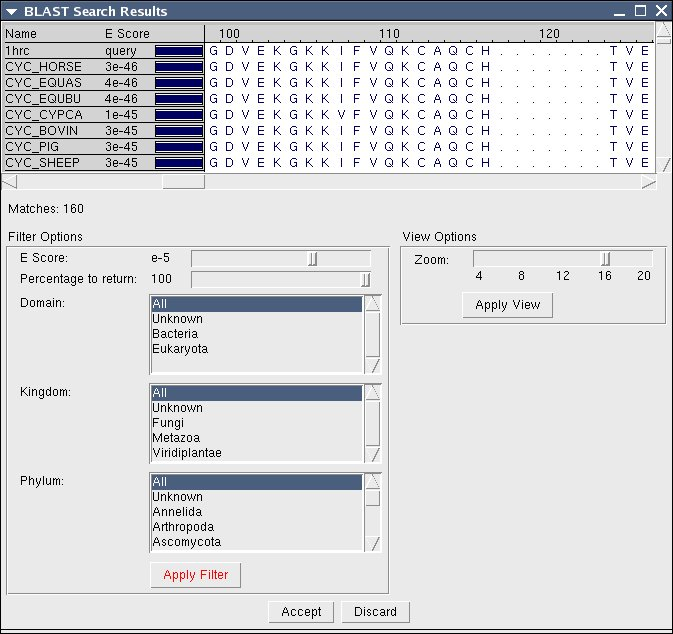
\includegraphics [width=5in]{./pictures/BLAST_results.jpg}}
 \caption{BLAST Search Results}%more information in caption about views etc.
\label{blast}
\end{figure}

MultiSeq will then begin a BLAST search.  This may take several minutes.
When the search is done, a new window called \textsf{BLAST Search
Results} will appear.  The results do not immediately appear in the main
MultiSeq window, because you can apply further filters on the retrieved
sequences.  The \textsf{BLAST Search Results} window is divided into
three main parts: the sequence viewer, \textsf{Filter Options}, and
\textsf{View Options}.     

The sequence viewer is a read-only display of the sequences that match
your BLAST search.  The number of matches is listed below the sequence
viewer.

You can use the \textsf{Zoom} to change how much of each sequence you
see.  You can change the zoom level and \textsf{Apply View} and you will
see fewer or more sequences in the sequence viewer portion of the
window.

In the \textsf{Filter Options} you can tweak the parameters to reduce or
expand the number of sequence matches.  Once you have changed a
parameter you can hit \textsf{Apply Filter} and see which sequences
match.

Once you have a collection of sequences that you want to import, you can
hit the \textsf{Accept} button at the bottom and they will be added to
the MultiSeq window.


